\chapter{Recurrences}

The generating series we have found are almost all \emph{rational functions}: quotients
$P(x)/Q(x)$ of polynomials. This chapter answers the natural question of how to get the
coefficients of a rational function, either as a recurrence or as an explicit formula.

\section{Coefficients of rational functions}

\begin{theorem}
Let $A(x) = \sum_{n\ge0} a_nx^n = \frac{P(x)}{Q(x)}$ where $P(x) = \sum p_nx^n$ is a polynomial and
$Q(x) = 1 + q_1x + q_2x^2 + \cdots + q_kx^k$. Then for all $n \ge 0$,
\[
a_n + q_1a_{n-1} + q_2a_{n-2} + \cdots + q_ka_{n-k} = p_n,
\]
where $a_j = 0$ for $j < 0$ and $p_n = 0$ for $n > \deg P$.
\end{theorem}
\begin{proof}
Compare the coefficient of $x^n$ on both sides of $Q(x)A(x) = P(x)$.
\end{proof}

So for $n > \max(\deg P, k-1)$ the coefficients satisfy the \emph{homogeneous} recurrence
$a_n = -q_1a_{n-1} - \cdots - q_ka_{n-k}$, and the first few values are fixed by $P$.

\begin{example}
For $\frac{1+x}{1-x-x^2}$: $a_n - a_{n-1} - a_{n-2} = p_n$ with $p_0 = p_1 = 1$. So $a_0 = 1$,
$a_1 = 1 + 1 = 2$, and $a_n = a_{n-1} + a_{n-2}$ for $n\ge2$: $1, 2, 3, 5, 8, 13,\dots$.
\end{example}

\begin{definition}[Linear recurrence]
A sequence satisfies a \emph{homogeneous linear recurrence with constant coefficients} of order
$k$ if
\[
a_n + q_1a_{n-1} + \cdots + q_ka_{n-k} = 0 \qquad (n \ge k)
\]
for constants $q_1,\dots,q_k$ with $q_k \ne 0$. The values $a_0,\dots,a_{k-1}$ are the
\emph{initial conditions}; they and the recurrence determine the sequence.
\end{definition}

Conversely, any such sequence has a rational generating series with denominator
$Q(x) = 1 + q_1x+\cdots+q_kx^k$ and a numerator of degree less than $k$ (multiply out
$Q(x)A(x)$ and observe all coefficients from $x^k$ on vanish).

\section{Partial fractions}

To get an explicit formula, factor the denominator. Over $\C$,
\[
Q(x) = (1 - \beta_1 x)^{m_1}(1 - \beta_2x)^{m_2}\cdots(1-\beta_jx)^{m_j}
\]
with distinct non-zero $\beta_i$ and $m_1 + \cdots + m_j = k$.

\begin{theorem}[Partial fractions]
If $\deg P < \deg Q$, there are constants $C_{i,r}$ such that
\[
\frac{P(x)}{Q(x)} = \sum_{i=1}^{j}\sum_{r=1}^{m_i}\frac{C_{i,r}}{(1-\beta_ix)^r}.
\]
\end{theorem}

Since $\coef{n}\frac{1}{(1-\beta x)^r} = \binom{n+r-1}{r-1}\beta^n$ and
$\binom{n+r-1}{r-1}$ is a polynomial in $n$ of degree $r-1$, this gives:

\begin{theorem}
If $A(x) = P(x)/Q(x)$ with $\deg P < \deg Q$ and $Q$ factored as above, then there are polynomials
$p_i(n)$ with $\deg p_i < m_i$ such that
\[
a_n = p_1(n)\beta_1^n + p_2(n)\beta_2^n + \cdots + p_j(n)\beta_j^n \qquad\text{for all } n\ge0.
\]
\end{theorem}

If $\deg P \ge \deg Q$, first divide: $P/Q = $ (polynomial) $+ R/Q$ with $\deg R < \deg Q$; then the
formula holds for $n > \deg P - \deg Q$.

\begin{example}
Find $a_n$ for $A(x) = \frac{2-x}{1-3x+2x^2}$. Factor $1 - 3x + 2x^2 = (1-x)(1-2x)$ and write
\[
\frac{2-x}{(1-x)(1-2x)} = \frac{a}{1-x} + \frac{b}{1-2x},\qquad 2-x = a(1-2x) + b(1-x).
\]
At $x = 1$: $1 = -a$, so $a = -1$. At $x = \frac12$: $\frac32 = \frac{b}{2}$, so $b = 3$. Hence
$a_n = 3\cdot2^n - 1$. Check: $a_0 = 2$, and the recurrence $a_n = 3a_{n-1} - 2a_{n-2} + p_n$
gives $a_1 = 3a_0 - 1 = 5$, and the formula gives $3\cdot 2 - 1 = 5$. Good.
\end{example}

\section{The characteristic polynomial}

It is usually quicker to skip partial fractions and work directly with the recurrence.

\begin{definition}[Characteristic polynomial]
The \emph{characteristic polynomial} of $a_n + q_1a_{n-1} + \cdots + q_ka_{n-k} = 0$ is
\[
C(x) = x^k + q_1x^{k-1} + \cdots + q_{k-1}x + q_k.
\]
\end{definition}

Note $C(x) = x^kQ(1/x)$, so $(1-\beta x)$ divides $Q(x)$ with multiplicity $m$ iff $\beta$ is a
root of $C(x)$ with multiplicity $m$. The roots of $C$ are the $\beta_i$ above, so:

\begin{theorem}[General solution]
If $C(x)$ has distinct roots $\beta_1,\dots,\beta_j$ with multiplicities $m_1,\dots,m_j$, then
every solution of the recurrence has the form
\[
a_n = \sum_{i=1}^{j}\left(c_{i,0} + c_{i,1}n + \cdots + c_{i,m_i-1}n^{m_i-1}\right)\beta_i^n,
\]
and the $k$ constants $c_{i,r}$ are determined by the $k$ initial conditions.
\end{theorem}

A quick sanity check of why this works for a simple root: $a_n = \beta^n$ satisfies the
recurrence iff $\beta^{n-k}(\beta^k + q_1\beta^{k-1} + \cdots + q_k) = 0$ iff $C(\beta) = 0$.

\begin{important}[Recipe]
\begin{enumerate}
  \item Write down $C(x)$ and find its roots with multiplicities.
  \item Write the general solution with unknown constants (a polynomial of degree $m-1$ in front
        of $\beta^n$ for a root of multiplicity $m$).
  \item Use the initial conditions to solve for the constants.
  \item Check the formula against one or two terms computed from the recurrence.
\end{enumerate}
\end{important}

\begin{example}[Distinct roots]
$a_n = 5a_{n-1} - 6a_{n-2}$, $a_0 = 1$, $a_1 = 4$. Then $C(x) = x^2 - 5x + 6 = (x-2)(x-3)$, so
$a_n = A\,2^n + B\,3^n$. From $A + B = 1$ and $2A + 3B = 4$: $B = 2$, $A = -1$, so
$a_n = 2\cdot3^n - 2^n$. Check: $a_2 = 5\cdot4 - 6 = 14 = 18 - 4$.
\end{example}

\begin{example}[Repeated root]
$a_n = 4a_{n-1} - 4a_{n-2}$, $a_0 = 1$, $a_1 = 6$. Then $C(x) = (x-2)^2$, so
$a_n = (A + Bn)2^n$. From $a_0$: $A = 1$; from $a_1$: $2(1 + B) = 6$, $B = 2$. So
$a_n = (2n+1)2^n$. Check: $a_2 = 24 - 4 = 20 = 5 \cdot 4$.
\end{example}

\begin{example}[Order three]
$a_n = 3a_{n-2} - 2a_{n-3}$ with $a_0 = 1$, $a_1 = 0$, $a_2 = 8$. Then
$C(x) = x^3 - 3x + 2 = (x-1)^2(x+2)$, so $a_n = A + Bn + D(-2)^n$. The initial conditions give
\[
A + D = 1,\qquad A + B - 2D = 0,\qquad A + 2B + 4D = 8.
\]
Subtracting the first from the other two: $B - 3D = -1$ and $2B + 3D = 7$, so $3B = 6$, $B = 2$,
$D = 1$, $A = 0$. Thus $a_n = 2n + (-2)^n$. Check: $a_3 = 3\cdot0 - 2\cdot1 = -2 = 6 - 8$ and
$a_4 = 3\cdot8 - 0 = 24 = 8 + 16$.
\end{example}

\begin{example}[Fibonacci numbers]
Compositions of $n$ with parts $1$ and $2$ satisfy $c_n = c_{n-1} + c_{n-2}$, $c_0 = c_1 = 1$.
$C(x) = x^2 - x - 1$ has roots $\phi = \frac{1+\sqrt5}{2}$ and $\psi = \frac{1-\sqrt5}{2}$, and
solving $A + B = 1$, $A\phi + B\psi = 1$ gives
\[
c_n = \frac{1}{\sqrt5}\left(\phi^{n+1} - \psi^{n+1}\right).
\]
Since $\abs{\psi} < 1$, $c_n$ is the nearest integer to $\phi^{n+1}/\sqrt5$; the number of such
compositions grows like $1.618^n$.
\end{example}

The recurrence itself is visible if we draw a composition with parts $1$ and $2$ as a tiling
of a $1\times n$ strip by squares and dominoes: the last tile is a square (leaving a strip of
length $n-1$) or a domino (leaving length $n-2$). The five tilings of length $4$:
\begin{center}
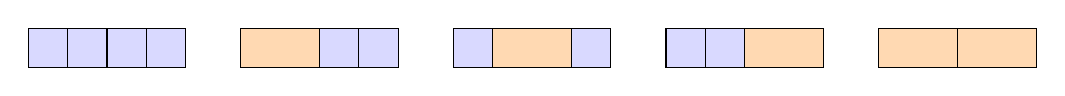
\begin{tikzpicture}[x=0.5cm,y=0.5cm]
  \foreach \t [count=\r from 0] in {{1,1,1,1},{2,1,1},{1,2,1},{1,1,2},{2,2}} {
    \begin{scope}[xshift=\r*2.7cm]
      \def\pos{0}
      \foreach \p in \t {
        \pgfmathsetmacro{\e}{\pos+\p}
        \ifnum\p=1 \draw[fill=blue!15] (\pos,0) rectangle (\e,1); \else \draw[fill=orange!30] (\pos,0) rectangle (\e,1); \fi
        \global\let\pos\e
      }
    \end{scope}
  }
\end{tikzpicture}
\end{center}

\section{Non-homogeneous recurrences}

A recurrence with an extra term depending on $n$ can be handled by generating series.

\begin{example}[Tower of Hanoi]
$a_n = 2a_{n-1} + 1$ for $n\ge1$, $a_0 = 0$. Multiply by $x^n$ and sum over $n \ge 1$:
\[
A(x) - a_0 = 2xA(x) + \frac{x}{1-x}\quad\Longrightarrow\quad
A(x) = \frac{x}{(1-x)(1-2x)} = \frac{1}{1-2x} - \frac{1}{1-x}.
\]
So $a_n = 2^n - 1$.
\end{example}

This recurrence comes from the puzzle: to move $n$ discs to another peg, move the top
$n-1$ out of the way ($a_{n-1}$ moves), move the largest disc ($1$ move), then move the $n-1$
discs back on top of it ($a_{n-1}$ moves).
\begin{center}
\begin{tikzpicture}[scale=0.55,>={Stealth}]
  \foreach \s/\t in {0/{start},9/{after $a_{n-1}$ moves}} {
    \begin{scope}[xshift=\s cm]
      \fill[gray!60] (-0.5,-0.2) rectangle (7.5,0);
      \foreach \p in {0,3.5,7} { \draw[very thick,gray] (\p,0) -- (\p,3); }
      \node[font=\scriptsize] at (3.5,-0.7) {\t};
    \end{scope}
  }
  \draw[fill=red!40] (-1.4,0) rectangle (1.4,0.5);
  \foreach \w [count=\k] in {1.1,0.85,0.6} { \draw[fill=blue!25] (-\w,0.5*\k) rectangle (\w,0.5*\k+0.5); }
  \node[font=\scriptsize] at (0,3.4) {$n$ discs};
  \begin{scope}[xshift=9cm]
    \draw[fill=red!40] (-1.4,0) rectangle (1.4,0.5);
    \foreach \w [count=\k] in {1.1,0.85,0.6} { \draw[fill=blue!25] (3.5-\w,0.5*\k-0.5) rectangle (3.5+\w,0.5*\k); }
    \draw[->,thick,red!70!black] (0,1) to[bend left=40] node[above,font=\scriptsize] {$1$ move} (7,0.8);
    \node[font=\scriptsize] at (3.5,2.2) {$n-1$};
  \end{scope}
\end{tikzpicture}
\end{center}

\section{Summary}
\begin{itemize}
  \item Coefficients of $P/Q$ with $Q = 1 + q_1x+\cdots+q_kx^k$ satisfy
        $a_n + q_1a_{n-1}+\cdots+q_ka_{n-k} = p_n$.
  \item Partial fractions give $a_n = \sum_i p_i(n)\beta_i^n$, $\deg p_i < m_i$.
  \item Characteristic polynomial $C(x) = x^kQ(1/x)$; its roots are the $\beta_i$.
  \item Always solve for constants with initial conditions and check against the recurrence.
\end{itemize}
